% !TEX encoding = UTF-8 Unicode
% !TEX program = pdflatex
% !TEX spellcheck = en_US


% In order to correctly compile this document,
% execute the following commands:
% 1. pdflatex
% 2. pdflatex
% 3. pdflatex



\documentclass[amsthm,ebook]{saparticle}

% IF YOU USE PDFLATEX
\usepackage[utf8x]{inputenc}
% if you write in english and in greek
\usepackage{ucs}
\usepackage[greek,english]{babel}
\languageattribute{greek}{polutoniko}

% IF YOU USE XELATEX
%\usepackage{polyglossia}
% if you write in italian
%\setmainlanguage{italian}
% If you want put some ancient greek:
%\setotherlanguage[variant=polytonic]{greek}
%\newfontfamily{\greekfont}[Ligatures=TeX]{Palatino Linotype}

% dummy text (remove in a normal thesis)
% remove if not necessary
\usepackage{siunitx}
%Natbib for bibliography management
\usepackage[authoryear]{natbib}
% custom commands
\newcommand{\bs}{\textbackslash}

%%%%%%%%
%TITLE:%
%%%%%%%%
\title{Searching inscriptions through the EAGLE Portal}

%%%%%%%%
%AUTHORS:%
%%%%%%%%
\author[PROMOTER]{Claudio Prandoni\corref{first}}
% put the label for the address (like FENWAY here) in the square brackets; change the addresses below to match the labelled authors
% mark the corresponding author with the \corref command and fill out the complete address in the \cortext command below

\author[PROMOTER]{Antonella Fresa}
\author[Gogate]{Nicola Alfarano}
\author[ISTI]{Giuseppe Amato}
\author[ISTI]{Franco Zoppi}
\author[ISTI]{Andrea Mannocci}
\author[HEI]{Pietro Liuzzo}
\author[DAI]{Francesco Mambrini}
\author[ROME]{Silvia Orlandi}
\author[ROME]{Raffaella Santucci}
%Promoter Srl1, Gogate Srl2, CNR-ISTI3, Heidelberg University4, German Archeological Institute5, Sapienza University of Rome6


%\author[ENEA]{Francesco Biccari}

%Additional information about corresponding author, addresses and affiliations:
\cortext[first]{Corresponding author. Email:  prandoni@promoter.it}

\address[PROMOTER]{Promoter Srl, Via Boccioni 2, 56037 Peccioli, Italy}
\address[Gogate]{Gogate Srl, Via Malasoma 24, 56121 Ospedaletto, Italy}
\address[ISTI]{CNR-ISTI, Via G. Moruzzi 1, 56124 Pisa, Italy }
\address[HEI]{Ruprecht-Karls-Universität Heidelberg, Marstallstraße 6, 69117, Heidelberg (DE)}
%\address[ENEA]{ENEA, Casaccia Research Center, via anguillarese 301, 00123 Roma, Italy}
\address[DAI]{Deutsches Archäologisches Institut, 69-71 Podbielskiallee, 14195 Berlin, Germany}
\address[ROME]{La Sapienza University of Rome, Piazzale Aldo Moro 5, 00185 Roma }

%%%%%%%%%%%%
%PAPER CONTENT %
%start your paper here%
%%%%%%%%%%%%

\begin{document}

\maketitle

\begin{abstract}
This paper describes the functionalities and the technical infrastructure of the EAGLE Portal, the main
gateway into the EAGLE’s massive epigraphic database. The portal can be accessed both by a human through a web browser
and by external applications through a set of APIs. It is possible to perform full-text searches using a simple
interface, or to launch more advanced queries, including the possibility to upload an image and search for inscriptions
that are similar to the provided one. The seven controlled multilingual vocabularies that were created to help aligning
the multilingual metadata of the inscriptions from the different content providers, have been also integrated in the
search engine as well as all the translations the are available on the EAGLE MediaWiki. All this makes of the EAGLE
Portal a very useful tool for the epigraphic community but also for single users and enthusiasts willing to contribute
to the research in this field.
\end{abstract}

\keywords{Search engine, API, image recognition, controlled vocabulary, multilingual translations, advanced search, citizen
participation}

\section{Introduction}

\noindent The EAGLE Portal is the place where the content provided by the epigraphers' community is aggregated and stored and
where it is made accessible to the users. It is composed by:

\begin{itemize}
\item The Metadata Aggregation System (in the following referred also as Aggregator), which is where all the content is
stored and indexed.
\item A Graphical User Interface (GUI), which is the interface through which users can browse the content and interact
with it.
\end{itemize}
The Aggregator relies on the D-NET software toolkit, developed within the DRIVER project and extended within the
OpenAIRE, OpenAIREplus\footnote{\url{http://www.openaire.eu/}}, EFG, EFG1914\footnote{\url{http://www.europeanfilmgateway.eu/it}}
and HOPE\footnote{\url{http://www.peoplesheritage.eu/}} projects. D-NET is an open source, general-purpose software conceived
to enable the realization and operation of Aggregative Data Infrastructures (ADIs) and to facilitate their evolution
and maintenance over time. D-NET implements a service-oriented framework based on standards, namely Web Services with
SOAP and REST APIs, where ADIs can be constructed in a LEGO-like approach, by selecting, customizing, and properly
combining D-NET services as building blocks. The resulting ADIs are systems, which can be customized, further extended
(e.g. by the integration of new services), and scaled (e.g. storage and index replicas can be maintained and deployed
on remote nodes to tackle multiple concurrent accesses or very-large data size) at run-time \citep{amato_aim_2013}.

The GUI exposes all the content stored in the Aggregator providing to the users the following functionalities \citep{prandoni_eagle_2014}.

\begin{itemize}
\item Search and browse the rich set of data made available by EAGLE content providers by using either a free text
search or a more advanced interface, including faceted browsing through the integration of the EAGLE controlled
vocabularies.
\item Similarity search through the image recognition algorithm that have been integrated in the EAGLE Portal.
\item Access to all the peer-reviewed translations of the epigraphic texts, in several European languages that have been
produced and integrated in the EAGLE MediaWiki.
\item Export to the user own PC the EpiDoc document of an object for further analysis and processing.
\item Annotate and save relevant information in a user Personal Space (e.g. records of inscriptions, search results,
queries), including content saved while using the Flagship Mobile Application.
\item Access to the Flagship Storytelling Application to browse the existing epigraphy-related narratives and to create
a new story.
\end{itemize}
The ingestion and curation of data is performed through a separate dedicated interface made available by the Aggregator.
This interface includes a series of functionalities to support data ingestion and storage as well as for importing,
indexing, enriching and managing the harvested metadata \citep{amato_second_2015}.

\section{The EAGLE Collections}

\noindent Classical Greek and Latin culture is at the very foundation of modern European identity. From philosophy to
architecture, geometry to law, a variety of contemporary subjects and disciplines have their roots in the classical
world. Only a small fraction of the total production of Greco-Roman texts has survived to the present day, leaving wide
gaps in the historiographical record of an epoch that is immensely relevant to our modern day lives. 

The collections held by the EAGLE partners have been assembled with the two-fold criterion of historical-cultural
significance and strong thematic unity. They feature a great variety of inscriptions written in Greek, Latin and other
ancient languages, providing scholars with an authoritative resource by which to verify the reliability of historical
reconstructions. Additionally, they equip the broad public with a way to understand and easily appreciate interesting
and geographically dispersed inscriptions.

The EAGLE collections come from a wide range of digital repositories of epigraphic content. The following paragraphs
illustrate these repositories.

Arachne\footnote{\url{http://arachne.uni-koeln.de}} is the central object-database of the German Archaeological Institute
(DAI). Since 2001, Arachne has been integrating negative archives of ancient sculpture that went beyond the specialised
documentation retained in Cologne itself, such as the negatives of ancient sculpture of the German Archaeological
Institute in Rome and the historic glass plate negative collections. Besides this larger project, many additional
activities are going on different levels, for example the online preparations for the »Corpus der Antiken
Sarkophagreliefs«.

Archaia Kypriaki Grammateia Digital Corpus (AKGDC) is a searchable digital library based on the 6 volumes of Archaia
Kypriaki Grammateia (Ancient Cypriot Literature), published by the A. G. Leventis Foundation between 1995-2008. The
AKGDC/ STARC collection of Cypriot inscriptions are dated from the 5th century BC to the 5th century AD and are mostly
funerary or dedicatory epigrams in elegiac couplet or hexameter.

Epigraphic Database Bari (EDB)\footnote{\url{http://www.edb.uniba.it}} is a project specialized in epigraphic documents of
Christian patronage (third to eighth centuries, AD), including those contained in the \emph{Inscriptiones Christianae Vrbis
Romae, nova series}, voll. I-X, in civitate Vaticana 1922-1992 (= ICVR), and those edited in other bibliographical seats
and/or not contained in the ICVR. Currently the inscriptions present in the EDB (counting those already online and
those awaiting definitive approval) amount to 40,000 items ca, though this number is obviously increasing continually. 

The task of the Epigraphic Database Heidelberg (EDH)\footnote{\url{http://edh-www.adw.uni-heidelberg.de}} is the systematic
entry of ancient Latin and bilingual (usually Latin and Greek) inscriptions into a complex database. The Epigraphic
Text Database is the heart of EDH and contains 65,000 inscriptions at present. Almost all of the records present texts,
which have already either been edited in the monumental Inscription corpora or published, revised and discussed in
thousands of scholarly articles.

Epigraphic Database Rome (EDR)\footnote{\url{http://edr-edr.it}} was launched in 1999 as an experimental project aimed at
creating a unified database for ancient epigraphy. EDR is part of the international federation of Epigraphic Databases
called Electronic Archive of Greek and Latin Epigraphy. The federation’s purpose is to collect all published Greek and
Latin inscriptions up to the 7th century A.D. considering their best existing editions, also enclosing, when possible,
a number of additional important data and/or images. As part of the federation, EDR aims at collecting the whole
epigraphy of Rome and of the Italian peninsula including Sardinia and Sicily, with the exception of Christian
inscriptions (under EDB jurisdiction).

Hispania Epigraphica Online\footnote{\url{http://eda-bea.es}} was created in 2002 when an EU grant enabled a joint research
project between the Archivo Epigráfico de Hispania and Mag. K. Schaller, who was developing computing applications for
archaeological purposes. The focus of the collection is the rich epigraphic patrimony of Portugal and Spain, mainly
written in Latin, but with some small pockets of Greek, Semitic and Iberian inscriptions.

Petrae database\footnote{\url{http://petrae.tge-adonis.fr}} is a system for the recording of Latin and Greek inscriptions
developed at the Institut Ausonius, which collects epigraphic texts from the various regions in which its researchers
and collaborators are active. Each record produced has the text of an inscription in both an uppercase and lowercase
version, accompanied by metadata on all aspects of the monument, including support, fragments, epigraphic fields and
text elements (dating, paleography, critical apparatus, translation, notes).

The Last Statues of Antiquity\footnote{\url{http://laststatues.classics.ox.ac.uk}} is a project funded in 2009 by the ‘Arts
and Humanities Research Council’ in Oxford. The project collects and analyses all the evidence for new, newly
dedicated, or newly re-worked statuary in the period \textit{circa} 284–650. The two main results of the project are a major
database, with over 2600 individual entries, and a book, published in late 2012, discussing in print the entire
phenomenon of the late-antique statue habit.

The picture database VBI ERAT LUPA\footnote{\url{http://www.ubi-erat-lupa.org}} contains stone monuments (sculptures,
reliefs, inscriptions, architectural pieces etc.). The project’s scope ranges from prehistoric stone monuments to
around the time of Justinian (500 AD). Due to its inception in Vienna, most project data at the moment is from the mid-
and south-eastern European region.

Finally, thanks to the great effort in the networking activities, many other partners joined the EAGLE Best Practice
Network and made available their collections that are currently being uploaded in the EAGLE Portal\footnote{ For a full
list of the EAGLE Associated Partners see \url{http://www.eagle-network.eu/about/partners/}}. 

\section{The EAGLE inscription search engine}

\noindent The EAGLE Inscriptions Search Engine is accessible through the main horizontal navigation bar of the EAGLE
Portal\footnote{\url{http://www.eagle-network.eu/basic-search/}}. It represents the core functionality of the portal,
through which the entry of keywords and phrases produce matches from EAGLE’s massive epigraphic database.

The EAGLE Portal makes available a ``simple search'', an ``advanced search'' where the user can specify the values of a
number of fields in order to make a more accurate search, and an ``image search'' where the user can upload an image and
search for inscriptions that look similar to the provided one \citep{prandoni_eagle_2014}. 

The objects that a user can search in the EAGLE Portal belong to three different categories, in accordance with the
EAGLE conceptual model \citep{sicilia_eagle_2015}:

\begin{itemize}
\item ``Artefacts'', which contain all the information that is somehow related to the physical carrier of the inscription.
\item ``Texts'', which contain all the information that is textual in nature.
\item ``Images'', which contain all the information that is visual in nature.
\end{itemize}

\subsection{How to search inscriptions}

\noindent The simple search user interface is very straightforward. The text entered in the query box is used to make a full text
search in all the fields of all the EAGLE objects in the category determined when making the query. By default, the
search will be done on all the objects in the ``Artefact'' category. Two more tabs on the result list (labelled ``Texts''
and ``Images'') allow the user to perform the same query choosing a different category.

Using the advanced search interface, a user can specify values for a number of fields, in order to have more accurate
results: findspot, bibliography, text of the inscription, type of inscription, decoration, object type, material, type
of writing, state of preservation (Fig. \ref{fig:figure1}).

In the fields having a controlled vocabulary, the user is allowed to enter only values coming from the vocabulary. For
this purpose, those fields have a ``drop-down menu'' which displays all the defined values for that field in the
``preferred label'', i.e. the text string that has been indicated in the vocabulary as the preferred one for display,
regardless of the language in which the string is defined. 

Finally, by choosing the Image Search option, a user can exploit the image recognition algorithm that has been
integrated in the EAGLE Portal and that allows to search for images that are similar to the one a user has uploaded,
ranked in decreasing order of similarity (Fig. \ref{figure2}).

\begin{figure}[!bp]
\centering
 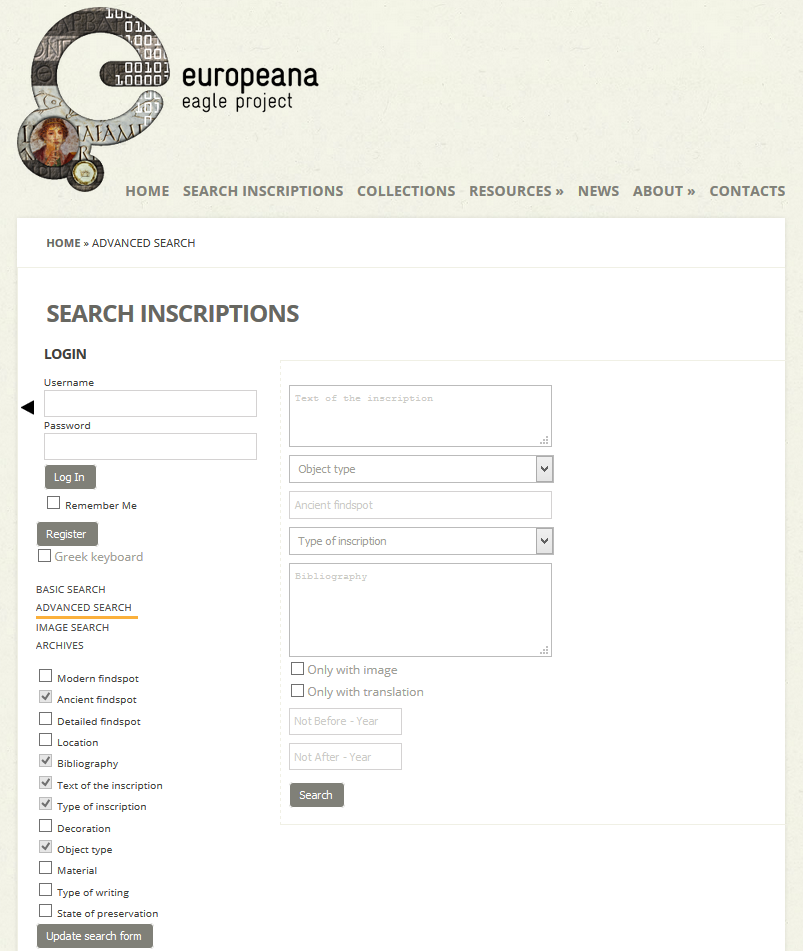
\includegraphics[width=10.874cm,height=12.885cm]{EAGLE2016submissionXX-img001.png} 
\caption{Search for inscriptions in the EAGLE Portal}
\label{fig:figure1}
\end{figure}

Content Based Image Retrieval (CBIR) is becoming an effective way for searching digital libraries, as the amount of
available image data is constantly increasing. CBIR applications are increasingly becoming useful in accessing cultural
heritage information, as a complement to metadata based search. In fact, in some cases metadata associated with images
do not describe the content with sufficient details to satisfy the user queries, or metadata are completely missing.
For example, images containing reproductions of works of art contain a lot of implicit information that is not
generally captured in manually or automatically generated metadata \citep{amato_aim_2013}.

The EAGLE Image Retrieval System (IRS) receives in input the image of an epigraph and provides effective and efficient
image similarity search and image content recognition of epigraphs.


\begin{figure}[!bp]
\centering
 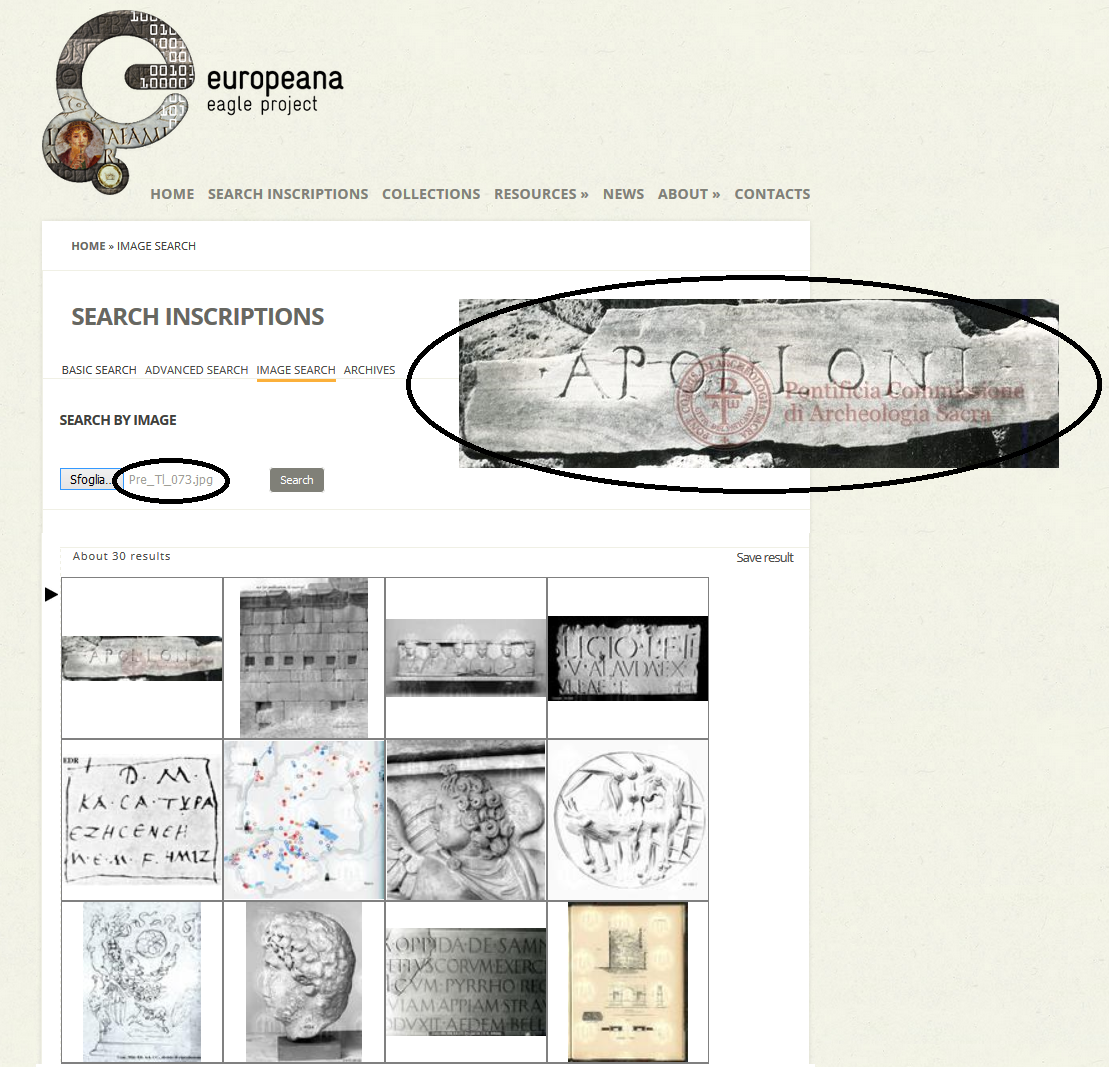
\includegraphics[width=10.848cm,height=10.451cm]{EAGLE2016submissionXX-img002.png} 
\caption{Image search in EAGLE}
\label{figure2}
\end{figure}

The images provided by the EAGLE content providers and collected in the Aggregator have been processed by a set of IRS
components (Image Feature Extractor, Image Indexer, CBIR Index) to build the index that allows a fast and efficient
similarity search during the query phase.

In addition, for those epigraphs where a set of images is available (training set), each training set has been processed
to extract the main features characterizing the epigraph. The training sets and the characterizing features are the
base for building another index, to be used by the image recognizer in order to decide if a received image (during the
query phase) can be classified as belonging to one of the existing sets or not. In this way, in many cases, the
recognizer is able to properly recognize the content of a query image even if the image given in the query was never
stored in the database.

\begin{figure}[!bp]
\centering
 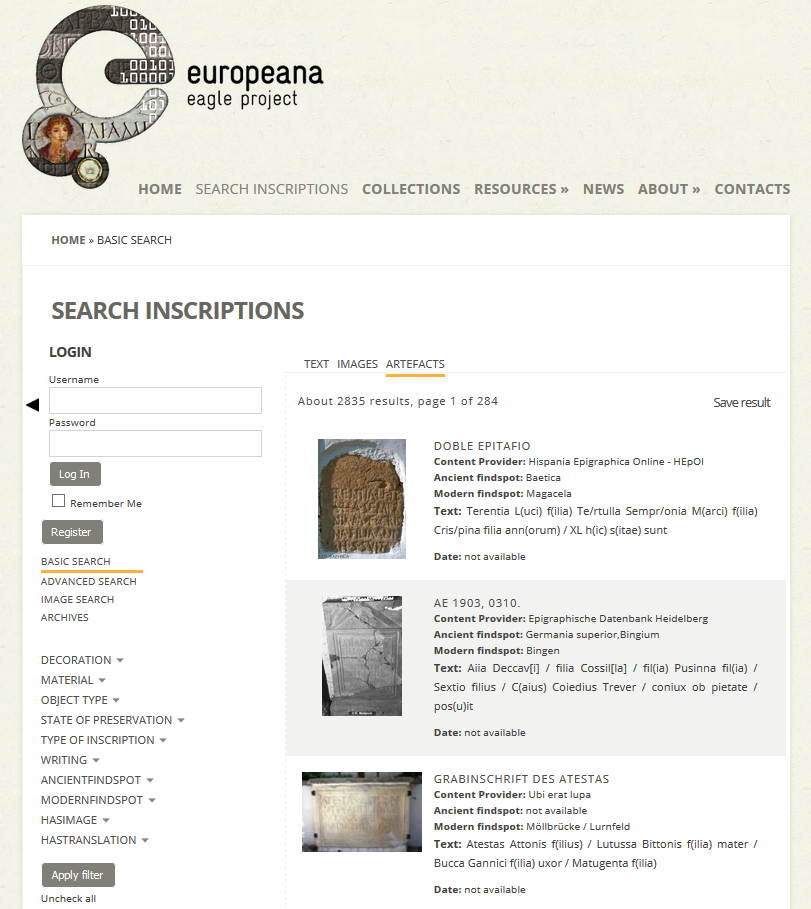
\includegraphics[width=10.874cm,height=12.197cm]{EAGLE2016submissionXX-img003.png} 
\caption{Results list - Artefacts}
\label{figure3}
\end{figure}

\subsection{Filtering and browsing results}

\noindent After having submitted a query, the user is presented with a paginated list of results containing some basic information (Fig. \ref{figure3}). 

By using the facets displayed on the left side panel, the user has the possibility to refine the query by applying some
filters based on the fields that are associated with a controlled vocabulary or based on the fact whether the
inscription has an image and/or a translation.

Regardless of the type of query performed by the user and of the category in which the query was done, clicking on one
of the items in the result page will display a summary of all the information available for that item, with links to
get further details (Fig. \ref{figure4}).

\begin{figure}[!bp]
\centering
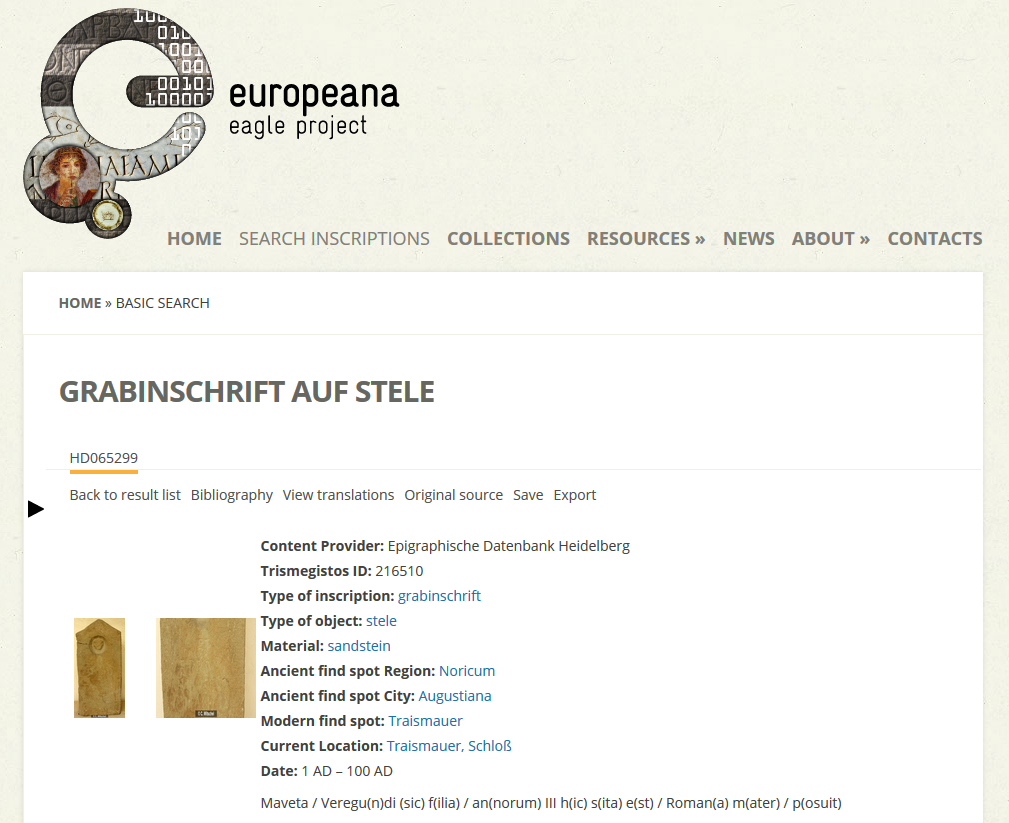
\includegraphics[width=10.874cm,height=8.864cm]{EAGLE2016submissionXX-img004.png}
\caption{Object details}
\label{figure4}
\end{figure}

The text in big characters on top of the page is the Title of the object. Below the title there is the local ID of the
object and after that there is a line collecting all the clickable items of the summary page: Bibliography, which opens
a text box with the bibliography associated with the object; Translations, which displays all the translations
available for the inscription of the object; Original source, which links the page of the object in the database of the
Content Provider who provided it; Save, which allows to save the object in the user’s personal space; Export, which
allows to download locally the EpiDoc document describing the object. Finally, all available pictures are displayed,
together with the remaining descriptive metadata.

Duplicates identification has been performed through the Trismegistos platform\footnote{\url{http://www.trismegistos.org/}}.
By standardizing publication references, collection information, material, provenance and date, the overlap of the
various databases has been mapped to identify records describing the same inscription. Afterwards a unique numeric
identifier, the Trismegistos ID, has been assigned to each document and spread across the partner databases for
inclusion in the metadata record to be uploaded in the EAGLE Portal.

If more than one instance of an object is available, the other instances appear on the summary page as clickable ``tabs'',
each tab being labelled with the local ID of the other instances of the same object.

The seven controlled multilingual vocabularies that have been created (Type of Inscription, Object Type, Material,
Execution, Decoration, State of Preservation, Dating Criteria) to help aligning the multilingual metadata of the
inscriptions from the different content providers, have been also integrated in the EAGLE search engine. Every time
that a term which belongs to one of the vocabularies is displayed, it is automatically linked to the specific page
describing the term, where further connections, synonyms and translations can be explored. The EAGLE vocabularies are
accessible also as Linked Open Data\footnote{\url{http://www.eagle-network.eu/resources/vocabularies/}}.

Finally, all the peer-reviewed translations in several European languages that are available, have been integrated in
the EAGLE Portal too through a RESTful API native of Wikibase, the MediaWiki extension used for this purpose\footnote{\url{http://www.eagle-network.eu/wiki/api.php}}. For each inscription it is possible to view the existing translation, to
request a new one and to contribute by connecting to the EAGLE MediaWiki\footnote{\url{http://www.eagle-network.eu/wiki}}.

\subsection{Annotating and saving objects}

A registered user, during a ``web'' or a ``mobile'' session, has the capability of annotating and saving (some of) the
information that is being provided by the EAGLE system.

Depending on the information the user is looking at, hitting the save button will save two types of data in the personal
space: 

\begin{itemize}
\item A query and its results.
\item Detailed information about an inscription.
\end{itemize}
The data saved by the local user on the EAGLE server is stored internally in a relational database.

A registered user logged in at the EAGLE Portal can access his/her saved data and perform some simple operations on it:

\begin{itemize}
\item Display of the saved queries or objects.
\item Modify the textual annotations associated with the saved item.
\item Delete the saved item from her personal space.
\item View the saved item.
\item Import the data that he/she saved during a mobile session.
\end{itemize}
It has to be noted that, when a user views one of the saved items, the object is displayed exactly as he/she saved it.
The saved data might be different from the data that can be retrieved by issuing the same query at the time of editing,
due to changes in the data stored in the EAGLE database. This allows the user to make comparisons between the
information that was available when he/she first saved the object and what has been added afterwards.

\section{Conclusion}

This paper presented the main functionalities of the EAGLE Portal, giving some highlights of the content that is
available and of the technical infrastructure that allows to search and browse them.

EAGLE aims to build a multi-lingual online collection of millions of digitised items from European museums, libraries,
archives and multi-media collections, which deal with inscriptions from the Greek and Roman World. The aim of the
network is to make available the vast majority of the surviving inscriptions of the Greco-Roman world, completed with
the essential information about them, enriched through the use of seven multilingual vocabularies, and complemented
with a series of peer-reviewed translations in several European languages, which are notoriously unavailable for
inscriptions. 

All this makes of the EAGLE Portal a very useful tool for the epigraphic community but also for single users and
enthusiasts willing to contribute to the research in this field.

The participation of Europe’s citizens in scientific research represents an important opportunity for improving European
competitiveness, because of the value that citizens can add in specific areas of research. In particular, the
participation of citizens in the research on CH and humanities has the potential to play an important role in the
development of the European Research Area, and can take the lead in the discovery of new directions of
cross-disciplinary research.

In this framework, the CIVIC EPISTEMOLOGIES\footnote{\url{http://www.civic-epistemologies.eu}} project developed a Roadmap
for the use of e-Infrastructures to support the participation of European citizens in CH practices and humanities
research, where such engagement has a twofold benefit for culture: to be enriched by the citizens’ contributions and to
become more widely used and exploited (also, for example, with the participation of creative industries) \citep{fresa_roadmap_2015}. The future development of the EAGLE initiative will refer to the CIVIC EPISTEMOLOGIES Roadmap for
investigating how to put in place more advanced services supporting citizen science in epigraphic research.

The EAGLE Portal is only an example of application that makes use of the APIs provided by the Aggregator to access the
EAGLE collections. Other examples are the Flagship Mobile Application\footnote{\url{http://www.eagle-network.eu/resources/flagship-mobile-app/}}, that allows to access the inscriptions’ database through
a mobile device and to fully exploit the image recognition features integrated in the EAGLE Portal, and the Flagship
Storytelling Application\footnote{\url{http://www.eagle-network.eu/stories/}}, that allows a user to create stories
starting from the content available in EAGLE, Europeana and many other data sources.

Other applications may be created based on the APIs provided by the Aggregator, which uses a SOLR-base search engine
through which it is possible to search and browse the full set of content\footnote{ For further information see
\url{http://wiki.apache.org/solr/\#Search\_and\_Indexing}}. Furthermore, APIs are provided to register a new user, login and
perform an image-based search using the EAGLE image recognition algorithm.


\bibliographystyle{sapauth-eng}
\bibliography{../../EAGLE}

\end{document}

